\documentclass[xcolor={usenames,dvipsnames}]{beamer}

\usepackage[T1]{fontenc}
%\usepackage{totcount}
%\regtotcounter{section}
%\usepackage{multido}
\usepackage{verbatim}
\usepackage{listings}

\title{Introduction to Dependent Types}
\subtitle{Eagan Technology Unconference}
\author{Joseph Ching}
\date{September 22, 2015}

\usetheme{Antibes}
\usecolortheme{beaver}

% http://tex.stackexchange.com/questions/131515/show-hide-subsections-in-the-table-of-contents-of-a-beamer-presentation
%\newcommand{\mytableofcontents}[0]{
%  \multido{\I=1+1}{\totvalue{section}}{
%    \begin{frame}<beamer>
%      \setcounter{section}{\I}
%      \frametitle{Outline}
%      \tableofcontents[
%      currentsection,
%      sectionstyle=show/show,
%      subsectionstyle=show/show/hide,
%      ]
%    \end{frame}
%  }
%  \setcounter{section}{0}
%}
% http://tex.stackexchange.com/questions/108898/beamer-presentation-show-toc-at-beginning-of-unnumbered-subsection-subsection
%\AtBeginSection[
%{\frame<beamer>{\frametitle{Outline}
%    \tableofcontents[currentsection]}}
%]
%{\frame<beamer>{
%    \frametitle{Outline}
%    \tableofcontents[currentsection]}
%}
% https://www.sharelatex.com/learn/Beamer
\AtBeginSection[] {
  \begin{frame}
    \frametitle{Section Outline}
    \tableofcontents[
      currentsection,
      sectionstyle=show/hide,
      subsectionstyle=show/show/hide
    ]
  \end{frame}
}
\newcommand{\hkeyword}[1]{\textcolor{TealBlue}{\textsc{#1}}}
\newcommand{\hfunction}[1]{\textcolor{Green}{\textsc{#1}}}
\newcommand{\htycon}[1]{\textcolor{Blue}{\textsc{#1}}}
\newcommand{\hvalcon}[1]{\textcolor{Red}{\textsc{#1}}}
\newcommand{\hkind}[1]{\textcolor{Fuchsia}{\textsc{#1}}}
\newcommand{\hclass}[1]{\textcolor{Magenta}{\textsc{#1}}}
\newcommand{\htyfam}[1]{\textcolor{OliveGreen}{\textsc{#1}}}
\newcommand{\hcomment}[1]{\textcolor{Grey}{\textsc{#1}}}
\newcommand{\hother}[1]{\textcolor{Black}{\textsc{#1}}}

\lstdefinestyle{hask}{
  basicstyle=\ttfamily\scriptsize\color{Black},
  sensitive=true,
  morecomment=[l][\color{Gray}\ttfamily\tiny]{--},
  morecomment=[s][\color{Gray}\ttfamily\tiny]{\{-}{-\}},
  morestring=[b]",
  stringstyle=\color{Maroon},
  showstringspaces=false,
  numberstyle=\color{Red},
  numberblanklines=true,
  showspaces=false,
  breaklines=true,
  showtabs=false,
  moredelim=**[is][\color{TealBlue}]{@kw}{@},
  moredelim=**[is][\color{Green}]{@f}{@},
  moredelim=**[is][\color{Blue}]{@tc}{@},
  moredelim=**[is][\color{Red}]{@vc}{@},
  moredelim=**[is][\color{Fuchsia}]{@dk}{@},
  moredelim=**[is][\color{Magenta}]{@cc}{@},
  moredelim=**[is][\color{OliveGreen}]{@tf}{@},
  moredelim=**[is][\color{Maroon}]{@str}{@},
  moredelim=**[is][\color{Black}]{@o}{@},
  escapeinside={{@|}{@}},
  % Keywords
  emph=
  {[1]
    % as didn't make it due to a:as
    module,import,qualified,hiding,foreign,infix,infixr,infixl,
    where,let,in,case,of,if,then,else,do,rec,proc,forall,pi,
    type,newtype,data,family,class,instance,deriving,default
  },
  emphstyle={[1]\color{TealBlue}\textbf},
  % functions
  emph=
  {[2]
    placeholder
  },
  emphstyle={[2]\color{Green}},
  % type constructors
  emph=
  {[3]
    Char,String,Bool,Int,Integer,Double,Float,Ordering,Maybe,Either,IO,
    List, Vec
  },
  emphstyle={[3]\color{Blue}\textbf},
  emph=
  % value constructors
  {[4]
    True,False,Nothing,Just,Left,Right,GT,LT,EQ,
    Nil, Cons, VNil, VCons
  },
  emphstyle={[4]\color{Red}\textbf},
  % type classes, contexts, constraints
  emph=
  {[5]
    Show,Read,Eq,Ord,Enum,Bounded,Num,
    Monoid,Functor,Foldable,Traversable,Applicative,Alternative,Monad,Comonad,Arrow
  },
  emphstyle={[5]\color{Magenta}\textbf},
  % kinds
  emph=
  {[6]
    Constraint,AnyK,OpenKind,BOX
  },
  emphstyle={[6]\color{Fuchsia}\textbf},
  % type families
  emph=
  {[7]
    Plus,Mult
  },
  emphstyle={[7]\color{OliveGreen}\textbf},
  % foreign languages
  emph=
  {[8]
    enum, interface, new, static, switch, return
  },
  emphstyle={[8]\color{TealBlue}\textbf},
}

\begin{document}


%%%%%%%%%%%%%%%%%%%%%%%%%%%%%%%%%%%%%%%%%%%%%%%%%%%%%%%%%%%%%%%%%%%%%%%%%%%%%%%%
%%% Title Page
%%%%%%%%%%%%%%%%%%%%%%%%%%%%%%%%%%%%%%%%%%%%%%%%%%%%%%%%%%%%%%%%%%%%%%%%%%%%%%%%
\begin{frame}[plain]
  \titlepage
\end{frame}


%%%%%%%%%%%%%%%%%%%%%%%%%%%%%%%%%%%%%%%%%%%%%%%%%%%%%%%%%%%%%%%%%%%%%%%%%%%%%%%%
%%% Table of Content
%%%%%%%%%%%%%%%%%%%%%%%%%%%%%%%%%%%%%%%%%%%%%%%%%%%%%%%%%%%%%%%%%%%%%%%%%%%%%%%%
% Want to hide subsection slide by slide
\begin{frame}{Table of Contents}
  \tableofcontents[
    pausesections,
    sectionstyle=show,
    subsectionstyle=hide
  ]
\end{frame}
%\mytableofcontents


%%%%%%%%%%%%%%%%%%%%%%%%%%%%%%%%%%%%%%%%%%%%%%%%%%%%%%%%%%%%%%%%%%%%%%%%%%%%%%%%
%%% Preface
%%%%%%%%%%%%%%%%%%%%%%%%%%%%%%%%%%%%%%%%%%%%%%%%%%%%%%%%%%%%%%%%%%%%%%%%%%%%%%%%
\section{Preface}

\begin{frame}{Quick Question}
  How many are familiar with this topic?
\end{frame}

\begin{frame}{A Joke}
  This is not a \texttt{m-} tutorial.

  \pause

  Nor is it a \texttt{lens} tutorial
  \pause
  (aka the new new \texttt{m-} tutorial\ldots

  \pause
  \ldots because \texttt{arrows} \textit{were} the new \texttt{m-} tutorials).

\end{frame}


\begin{frame}{About This Talk}
    \texttt{Agda}, \texttt{Idris}, \texttt{Coq} and co$^*$ have full support for dependent types.

    \ \\
    \pause
    Because of that, it's harder to see the build up, so we won't be directly using them in this talk.
    \ \\
    \ \\
    \pause
    \textit{\tiny{Honestly though, it's because they're way over my head :(}}\\
    \textit{\tiny{(*) There was another mini joke here\ldots}}
\end{frame}

\begin{frame}{About This Talk}
  But we will be using \texttt{Haskell} though :)

  \ \\
  \pause
  It's not truely dependent, but we can do more and more with each \texttt{language extension} that comes along.\\

  \ \\
  \pause
  For the examples, there will also be \textit{very} loose translation to imperative/OOP. Though please keep in mind that these are merely syntax translations, the actual concepts can differ vastly.
\end{frame}


%%%%%%%%%%%%%%%%%%%%%%%%%%%%%%%%%%%%%%%%%%%%%%%%%%%%%%%%%%%%%%%%%%%%%%%%%%%%%%%%
%%% Introduction
%%%%%%%%%%%%%%%%%%%%%%%%%%%%%%%%%%%%%%%%%%%%%%%%%%%%%%%%%%%%%%%%%%%%%%%%%%%%%%%%
\section{Review of Basics}

%%%%%%%%%%%%%%%%%%%%%%%%%%%%%%%%%%%%%%%%%%%%%%%%%%%%%%%%%%%%%%%%%%%%%%%%%%%%%%%%
\subsection{Values and Types}

\begin{frame}[fragile]{Values and Types}
  \hvalcon{Values} has \htycon{Types}, or \hvalcon{Values} are classified by \htycon{Types}.\\

  \begin{lstlisting}[style=hask]
    @|\ldots@, @vc-1@, @vc0@, @vc1@, @vc2@, @vc3@, @|\dots@ :: Int @|\pause@

    True, False :: Bool @|\pause@

    @str'a'@, @str'b'@, @str'c'@ :: Char @|\pause@

    "abc" :: String @|$\sim$@ @tc[@Char@tc]@

  \end{lstlisting}

  \tiny{\hvalcon{Values} are also called \hvalcon{Terms}}
\end{frame}

\begin{frame}[fragile]{About Types}
  How are data types defined?\\
  \pause
  \begin{itemize}
    \item Some are built in magic: \htycon{Int}, \htycon{Char}, functions
    \pause
    \item Some are built in sugar: list, tuples
      \begin{itemize}
        \item We can define equivalent non-sugar version ourselves
      \end{itemize}
    \pause
    \item Rest can be user defined: \htycon{Bool}, \htycon{String}, \htycon{Maybe}
  \end{itemize}
\end{frame}

\begin{frame}[fragile]{About Types}
  What are the data types like?
  \pause
  \begin{itemize}
    \item Multiple \hvalcon{Value} constructors
    \pause
    \item Paremetrize over another type
    \pause
    \item Recursive definition
    \pause
    \item Synonyms of other types
    \pause
    \item A combination of the above
  \end{itemize}
\end{frame}

%%%%%%%%%%%%%%%%%%%%%%%%%%%%%%%%%%%%%%%%%%%%%%%%%%%%%%%%%%%%%%%%%%%%%%%%%%%%%%%%
\subsection{Defining Data Types}
\begin{frame}[fragile]{Defining Data Types}
  Define new data type with \hkeyword{data}.

  \pause
  \ \\
  \begin{itemize}
    \item Left hand side (\htycon{LHS}) - \htycon{Type} constructor
    \item Right hand side (\hvalcon{RHS}) - \hvalcon{Value} constructor
  \end{itemize}

  \pause
  \ \\
  \htycon{Type} and \hvalcon{Value} constructors are capticalized.
\end{frame}

\begin{frame}[fragile]{Our First Example!}
  Define a person:
  \begin{lstlisting}[style=hask]
    -- | params for firstname, lastname, age respectively
    data @tcPerson@ = @vcPerson@ String String Int
  \end{lstlisting}

  \pause
  A loose translation:
  \begin{lstlisting}[style=hask]
    enum @tcPerson@ {
      @vcPerson@(String firstname, String lastname, Int age)
    }
  \end{lstlisting}

  \pause
  In this example, the \htycon{Type} and \hvalcon{Value} constructor have the same name. The \htycon{Type} of the \hvalcon{Person} constructor:
  \begin{lstlisting}[style=hask]
    @vcPerson@ :: String -> String -> Int -> @tcPerson@

    bobby :: @tcPerson@
    bobby = @vcPerson@ "Bobby" "Smith" @vc23@ @|\pause@

    -- a loose translation:
    @tcPerson@ bobby = new @vcPerson@("Bobby", "Smith", 23)
  \end{lstlisting}
\end{frame}

\begin{frame}[fragile]{Multiple Value Constructors}
  Data can have multiple \hvalcon{Value} constructors:
  \begin{lstlisting}[style=hask]
    data Bool = False | True

    data @tcWeekdays@ = @vcSunday@ | @vcMonday@ | @vcTuesday@ | @vcWednesday@
                  | @vcThursday@ | @vcFriday@ | @vcSaturday@
  \end{lstlisting}
  \textit{\tiny{Does this remind you of anything?}}

  \pause
  \ \\
  A loose translation:
  \begin{lstlisting}[style=hask]
    enum Bool { False, True }

    enum @tcWeekdays@ {
      @vcSunday@, @vcMonday@, @vcTuesday@, @vcWednesday@, @vcThursday@, @vcFriday@, @vcSaturday@
    }
  \end{lstlisting}
\end{frame}

\begin{frame}[fragile]{Multiple Value Constructor}
  You can do type aliasing with \hkeyword{type}:
  \begin{lstlisting}[style=hask]
    type @tcSide@ = Double
    type @tcRadius@ = Double
  \end{lstlisting}

  \pause
  For example:
  \begin{lstlisting}[style=hask]
    data @tcShape@ = @vcTriangle@ @tcSide@ @tcSide@ @tcSide@
               | @vcRectangle@ @tcSide@ @tcSide@
               | @vcCircle@ @tcRadius@
  \end{lstlisting}

  \pause
  A loose translation:
  \begin{lstlisting}[style=hask]
    enum @tcShape@ {
      @vcTriangle@(Double side1, Double side2, Double side3),
      @vcRectangle@(Double length, Double width),
      @vcCircle@(Double radius)
    }
  \end{lstlisting}
\end{frame}

\begin{frame}[fragile]{Multiple Value Constructor}
  Recall \htycon{Side} $\sim$ \htycon{Radius} $\sim$ \htycon{Double}:
  \begin{lstlisting}[style=hask]
    data @tcShape@ = @vcTriangle@ @tcSide@ @tcSide@ @tcSide@
               | @vcRectangle@ @tcSide@ @tcSide@
               | @vcCircle@ @tcRadius@
  \end{lstlisting}

  \pause
  \htycon{Types} of the \hvalcon{Value} constructors:
  \begin{lstlisting}[style=hask]
    @vcTriangle@  :: @tcSide@ -> @tcSide@ -> @tcSide@ -> @tcShape@
    @vcRectangle@ :: @tcSide@ -> @tcSide@ -> @tcShape@
    @vcCircle@    :: @tcRadius@ -> @tcShape@
  \end{lstlisting}

  \pause
  Example \htycon{Shapes}:
  \begin{lstlisting}[style=hask]
    myTri, myRect, myCir :: @tcShape@
    myTri  = @vcTriangle@ @vc2.1 3.2 5@
    myRect = @vcRectangle@ @vc4 4@
    myCir  = @vcCircle@ @vc7.2@
  \end{lstlisting}
\end{frame}

\begin{frame}[fragile]{Parametrization}
  Types can parametrize over another type:
  \begin{lstlisting}[style=hask]
    data @tcIdentity@ a = @vcIdentity@ a
  \end{lstlisting}

  \pause
  A loose translation:
  \begin{lstlisting}[style=hask]
    enum @tcIdentity@<A> {
      @vcIdentity@(A a)
    }
  \end{lstlisting}

  \pause
  The \htycon{Type} of the \hvalcon{Identity} constructor:
  \begin{lstlisting}[style=hask]
    @vcIdentity@ :: a -> @tcIdentity@ a

    intIdwrtSum :: @tcIndentity@ Int
    intIdwrtSum = @vcIdentity@ @vc0@
  \end{lstlisting}
\end{frame}

\begin{frame}[fragile]{Tuple}
  Parametrize over 2 types - 2-tuple!
  \begin{lstlisting}[style=hask]
    data @tcTuple@ a b = @vcTuple@ a b
  \end{lstlisting}

  \pause
  A loose translation:
  \begin{lstlisting}[style=hask]
    enum @tcTuple@<A, B> {
      @vcTuple@(A a, B b)
    }
  \end{lstlisting}

  \pause
  With:
  \begin{lstlisting}[style=hask]
    @vcTuple@ :: a -> b -> @tcTuple@ a b
  \end{lstlisting}
\end{frame}

\begin{frame}[fragile]{Tuple}
  Actual built-in sugar:
  \begin{lstlisting}[style=hask]
       data @tcTuple@ a b = @vcTuple@ a b
    => data @tc(,)@ a b = @vc(,)@ a b
    => data @tc(@a@tc,@ b@tc)@ = @vc(@a@vc,@ b@vc)@
  \end{lstlisting}

  \pause
  An example:
  \begin{lstlisting}[style=hask]
    type @tcEmployed@ = Bool

    barbara, chet, luffy :: @tc(@@tcPerson@@tc,@ @tcEmployed@@tc)@
    barbara = @vc(@@vcPerson@ "Barbara" "Sakura" @vc30,@ True@vc)@
    chet    = @vc(@@vcPerson@ "Chet" "Awesome-Laser" @vc2,@ False@vc)@
    luffy   = @vc(@@vcPerson@ "Luff D." "Monkey" @vc19,@ False@vc)@
  \end{lstlisting}
\end{frame}

\begin{frame}[fragile]{Maybe}
  Like \htycon{Bool}, but parametrize an $a$ over the \htycon{True} part:
  \begin{lstlisting}[style=hask]
    data Maybe a = Nothing | Just a
  \end{lstlisting}

  \pause
  A loose translation:
  \begin{lstlisting}[style=hask]
    enum Maybe<A> {
      Nothing,
      Just(A a)
    }
  \end{lstlisting}

  \pause
  The \htycon{Types} of the two \hvalcon{Value} constructors:
  \begin{lstlisting}[style=hask]
    Nothing :: Maybe a
    Just    :: a -> Maybe a
  \end{lstlisting}
\end{frame}

\begin{frame}[fragile]{Maybe}
  From previous slide:
  \begin{lstlisting}[style=hask]
    data Maybe a = Nothing | Just a
  \end{lstlisting}

  \pause
  Say more with the occupation:
  \begin{lstlisting}[style=hask]
    type @tcOccupation@ = Maybe String

    barbara, chet, luffy :: @tc(@@tcPerson@@tc,@ @tcOccupation@@tc)@
    barbara = @vc(@@vcPerson@ "Barbara" "Sakura" @vc30,@ Just "dancer"@vc)@
    chet    = @vc(@@vcPerson@ "Chet" "Awesome-Laser" @vc2,@ Nothing@vc)@
    luffy   = @vc(@@vcPerson@ "Luff D." "Monkey" @vc19,@ Just "pirate"@vc)@
  \end{lstlisting}
\end{frame}

\begin{frame}[fragile]{Either}
  Like \htycon{Bool}, but parametrize over both \hvalcon{True} and \hvalcon{False}:
  \begin{lstlisting}[style=hask]
    data Either a b = Left a | Right b
  \end{lstlisting}

  \pause
  A loose translation:
  \begin{lstlisting}[style=hask]
    enum Either<A, B> {
      Left(A a),
      Right(B b)
    }
  \end{lstlisting}

  \pause
  The two \hvalcon{Value} constructors have \htycon{Types}:
  \begin{lstlisting}[style=hask]
    Left  :: a -> Either a b
    Right :: b -> Either a b
  \end{lstlisting}
\end{frame}

\begin{frame}[fragile]{Either}
  From previous slide:
  \begin{lstlisting}[style=hask]
    data Either a b = Left a | Right b
  \end{lstlisting}

  \pause
  Refine with more details:
  \begin{lstlisting}[style=hask]
    type @tcEarning@ = Either String Int

    barbara, chet, luffy :: @tc(@@tcPerson@@tc,@ @tcEarning@@tc)@
    barbara = @vc(@@vcPerson@ "Barbara" "Sakura" @vc30,@
              Right @vc100000@@vc)@
    chet    = @vc(@@vcPerson@ "Chet" "Awesome-Laser" @vc2,@
              Left "Is a baby"@vc)@ 
    luffy   = @vc(@@vcPerson@ "Luff D." "Monkey" @vc19,@
              Right @vc2000000@@vc)@
  \end{lstlisting}
\end{frame}

\begin{frame}[fragile]{Types with Recursion}
  Natural number:
  \begin{lstlisting}[style=hask]
    data @tcNat@ = @vcZ@ | @vcS@ @tyNat@

    @vcZ@ :: @tcNat@
    @vcS@ :: @tcNat@ -> @tcNat@
  \end{lstlisting}

  \pause
  A loose translation:
  \begin{lstlisting}[style=hask]
    enum @tyNat@ {
      @vcZ@,
      @vcS@(@tyNat@ n)
    }
  \end{lstlisting}
\end{frame}

\begin{frame}[fragile]{Types with Recursion}
  Natural number:
  \begin{lstlisting}[style=hask]
    data @tcNat@ = @vcZ@ | @vcS@ @tcNat@

    @vcZ@ :: @tcNat@
    @vcS@ :: @tcNat@ -> @tcNat@

    0 @|$\sim$@ @vcZ@
    1 @|$\sim$@ @vcS@ @vcZ@
    2 @|$\sim$@ @vcS@ (@vcS@ @vcZ@)
    3 @|$\sim$@ @vcS@ (@vcS@ (@vcS@ @vcZ@))
  \end{lstlisting}
\end{frame}

\begin{frame}[fragile]{Types with Recursion}
  List - recursive type while parametrize over another type:
  \begin{lstlisting}[style=hask]
    data List a = Nil | Cons a (List a)

    Nil :: List a
    Cons :: a -> List a -> List a
  \end{lstlisting}

  \pause
  A loose translation:
  \begin{lstlisting}[style=hask]
    enum List<A> {
      Nil,
      Cons(A a, List<A> as)
    }
  \end{lstlisting}
\end{frame}

\begin{frame}[fragile]{Types with Recursion}
  Actual built-in sugar is something like:
  \begin{lstlisting}[style=hask]
       data List a = Nil | Cons a (List a)
    => data @tc[]@ a = @vc[]@ | @vc(:)@ a (@tc[]@ a)
    => data @tc[@a@tc]@ = @vc[]@ | a @vc:@ @tc[@a@tc]@
  \end{lstlisting}

  \pause
  De-sugar that list:
  \begin{lstlisting}[style=hask]
    ints :: List Int 
    ints = Cons 1 (Cons 2 (Cons 3 (Cons 4 Nil)))

    -- built-in sugar
    ints :: @tc[]@ Int
    ints = 1 @vc:@ 2 @vc:@ 3 @vc:@ 4 @vc:@ @vc[]@

    -- 2x the sugar!
    ints :: @tc[@Int@tc]@
    ints = @vc[@1, 2, 3, 4@vc]@
  \end{lstlisting}
\end{frame}


%%%%%%%%%%%%%%%%%%%%%%%%%%%%%%%%%%%%%%%%%%%%%%%%%%%%%%%%%%%%%%%%%%%%%%%%%%%%%%%%
\subsection{Functions}

\begin{frame}[fragile]{Functions}
  Maps \hvalcon{Values} of a \htycon{Type} to another \htycon{Type}:
  \begin{lstlisting}[style=hask]
    even :: Int -> Bool
    even @vc0@ = True
    even n = if rem n 2 == @vc0@
             then True
             else False
  \end{lstlisting}

  \pause
  Not as loose translation:
  \begin{lstlisting}[style=hask]
    static Bool even (Int n) {
      switch n:
        case n == 0:
          return True;
        default:
          if rem(n, 2) == 0
            return True;
          else
            return False;
    }
  \end{lstlisting}
\end{frame}

\begin{frame}[fragile]{Functions with Recursion}
  Use recursion for recursive types:
  \begin{lstlisting}[style=hask]
    toInt :: @tcNat@ -> Int
    toInt @vcZ@     = @vc0@
    toInt (@vcS@ n) = @vc1@ + toInt n
  \end{lstlisting}

  \pause
  Not as loose translation:
  \begin{lstlisting}[style=hask]
    static Int toInt (@tcNat@ n) {
      switch n:
        case @vcZ@:
          return @vc0@;
        case (@vcS@ m):  -- n @|$\sim$@ (S m)
          return @vc1@ + toInt(m);
    }
  \end{lstlisting}
\end{frame}

\begin{frame}[fragile]{Type of Functions}
  Q: Actual type of functions?\\
  \pause
  A: Built-in magic, it's called the $function\ arrow$, something like:
  \begin{lstlisting}[style=hask]
    data (->) a b = implementation

    even  :: Int @tc->@ Bool
    toInt :: @tcNat@ @tc->@ Int
  \end{lstlisting}
\end{frame}

\begin{frame}[fragile]{Functions with Parametric Polymorphism}
  Functions can be parametric:
  \begin{lstlisting}[style=hask]
    id :: a -> a
    id a = a
  \end{lstlisting}

  \pause
  Not as loose translation:
  \begin{lstlisting}[style=hask]
    static A id<A>(A a) {
      return a;
    }
  \end{lstlisting}
\end{frame}

\begin{frame}[fragile]{Functions with Parametric Polymorphism}
  Functions can be parametric:
  \begin{lstlisting}[style=hask]
    append :: @tc[@a@tc]@ -> @tc[@a@tc]@ -> @tc[@a@tc]@
    append @vc[]@     ys = ys
    append (x@vc:@xs) ys = x @vc:@ append xs ys
  \end{lstlisting}

  \pause
  A translation:
  \begin{lstlisting}[style=hask]
    static List<A> append(List<A> l1, List<A> l2) {
      switch l1:
        case Nil:
          return l2;
        case Cons(x, xs):
          List<A> rest = append(xs, l2);
          return Cons(x, rest);
    }
  \end{lstlisting}
\end{frame}

\begin{frame}[fragile]{Higher-order Functions}
  Functions that take functions as params:
  \begin{lstlisting}[style=hask]
    -- actual name is ($)
    apply :: (a -> b) -> a -> b
    apply f x = f x

    -- acutal name is (.)
    compose :: (b -> c) -> (a -> b) -> (a -> c)
    compose f g = \x -> f (g x)
  \end{lstlisting}

  \pause
  Yay translations:
  \begin{lstlisting}[style=hask]
    static B apply(Func<A, B> f, A a) {
      return f(a);
    }

    static Func<A,C> compose(Func<B,C> f, Func<A,B> g) {
      return x => f(g(x));
    }
  \end{lstlisting}
\end{frame}

\begin{frame}[fragile]{More Functions Examples}
  $map$:
  \begin{lstlisting}[style=hask]
    map :: (a -> b) -> @tc[@a@tc]@ -> @tc[@b@tc]@
    map f @vc[]@     = @vc[]@
    map f (x@vc:@xs) = f x @vc:@ map f xs
  \end{lstlisting}

  \pause
  A translation:
  \begin{lstlisting}[style=hask]
    static List<B> map(Func<A,B> f, List<A> la) {
      switch la:
        case Nil:
          return Nil;
        case Cons(a, as):
          B b = f(a)
          List<B> rest = map(f, as);
          return Cons(b, rest);
    }
  \end{lstlisting}
\end{frame}

\begin{frame}[fragile]{More Functions Examples}
  $zip$:
  \begin{lstlisting}[style=hask]
    zip :: @tc[@a@tc]@ -> @tc[@b@tc]@ -> @tc[(@a@tc,@b@tc)]@
    zip @vc[]@     ys     = @vc[]@
    zip xs     @vc[]@     = @vc[]@
    zip (x@vc:@xs) (y@vc:@ys) = @vc(@x@vc,@y@vc)@ @vc:@ zip xs ys
  \end{lstlisting}

  \pause
  A translation:
  \begin{lstlisting}[style=hask]
    static List<@tcTuple@<A,B>> zip(List<A> l1, List<A> l2) {
      switch l1:
        case Nil:
          return Nil;
        case Cons(a, as):
          switch l2:
            case Nil:
              return Nil;
            case Cons(b, bs):
              @tcTuple@<A,B> front = @vcTuple@(a, b);
              List<@tcTuple@<A,B>> rest = zip(as, bs);
              return Cons(front, rest);
    }
  \end{lstlisting}
\end{frame}

%%%%%%%%%%%%%%%%%%%%%%%%%%%%%%%%%%%%%%%%%%%%%%%%%%%%%%%%%%%%%%%%%%%%%%%%%%%%%%%%
%%% Type Theory
%%%%%%%%%%%%%%%%%%%%%%%%%%%%%%%%%%%%%%%%%%%%%%%%%%%%%%%%%%%%%%%%%%%%%%%%%%%%%%%%
\section{What is Dependent Type}

%%%%%%%%%%%%%%%%%%%%%%%%%%%%%%%%%%%%%%%%%%%%%%%%%%%%%%%%%%%%%%%%%%%%%%%%%%%%%%%%
\subsection{$\lambda$-Calculus}

\begin{frame}[fragile]{$\lambda$-Calculus}
  So far, we have seen:
  \pause
  \begin{itemize}
    \item function application
    \item function abstraction {\tiny(aka higher-order functions)}
    \pause
    \item variable binding
    \pause
    \item substitution
  \end{itemize}
  \pause
  => basis for simply typed $\lambda$-calculus.
\end{frame}


\begin{frame}[fragile]{$\lambda$-Calculus}
  Q: Sure, but can we have more?
  \ \\
  \pause
  A: Yes, extend $\lambda$-calculus so we can have more forms of abstractions.

  \ \\
  \pause
  Q: But how?\\
  \pause
  A: What if I told you\ldots\\
  \pause
  \qquad \ldots you already know at least 2 axes of extension :)
\end{frame}


%%%%%%%%%%%%%%%%%%%%%%%%%%%%%%%%%%%%%%%%%%%%%%%%%%%%%%%%%%%%%%%%%%%%%%%%%%%%%%%%
\subsection{Extensions on $\lambda$-calculus}

\begin{frame}[fragile]{Subtype Polymorphism}
  Given data types \htycon{$T$} and \htycon{$P$}, if there is a relation between \htycon{$T$} and \htycon{$P$} by some notion of substitutability with \htycon{$T$} in place of \htycon{$P$}, then we say \htycon{$T$} is a \textit{subtype} of the \textit{supertype} \htycon{$P$}, denoted by \htycon{$T$} $<:$ \htycon{$P$}.

  \ \\
  \pause
  The name for this extension of $\lambda$-calculus is called \textit{subtype polymorphism} and is denoted by $\lambda_{<:}$.\\
  \pause
  => Object Oriented Programming.
  
  \ \\
  \pause
  Though this is not an axis that we are interested in.
\end{frame}

\begin{frame}[fragile]{Parametric Polymorphism}
  Introduce a mechanism of universal quantification over \htycon{Types}: \htycon{Types} can abstract over \htycon{Types}, allows for \textit{generic data types} and \textit{generic functions}.\\
  \pause
  => Generic Programming.

  \ \\
  \pause
  Recall:
  \begin{lstlisting}[style=hask]
    data @tc[@a@tc]@ = @vc[]@ | @vc(:)@ a @vc[@a@vc]@

    id :: a -> a
    map :: (a -> b) -> @vc[@a@vc]@ -> @vc[@b@vc]@
  \end{lstlisting}

  \pause
  The name for this extension is formally \textit{second order} $\lambda$\textit{-calculus}, aka \textit{System F}, denoted by $\lambda2$,
\end{frame}

\begin{frame}[fragile]{Value and Type Interdependency}
  Re-thinking functions:
  \begin{lstlisting}[style=hask]
    data Bool = False | True
    -- built-in magic: infinitely many value constructors
    data Int = ... | @vc-1@ | @vc0@ | @vc1@ | @vc2@ | ... 

    even :: Int -> Bool
    even @vc0@ = True
    even n = if rem n @vc2@ == @vc0@
             then True
             else False
  \end{lstlisting}

  \qquad f maps \hvalcon{numbers} to \hvalcon{True} and \hvalcon{False}.
  \ \\
  \pause
  => \hvalcon{Values} on RHS depends on the \hvalcon{Values} on LHS
  \ \\
  \pause
  => \hvalcon{Values} depending on \hvalcon{Values}
\end{frame}

\begin{frame}[fragile]{Value and Type Interdependency}
  Re-thinking parametrized data types:
  \begin{lstlisting}[style=hask]
    data Maybe a = Nothing | Just a

    data List a = Nil | Cons a (List a)
  \end{lstlisting}

  \pause
  \qquad \htycon{List} takes a \htycon{Type} and return \hvalcon{Value} constructors
  \ \\
  \pause
  => \hvalcon{Values} on RHS depends on the \htycon{Type} on LHS
  \ \\
  \pause
  => \hvalcon{Values} depending on \htycon{Types}
  \ \\
  \pause
  => Parametric polymorphism of $\lambda2$ again

  \ \\
  \pause
  \textit{\tiny{Are we seeing a pattern yet?}}
\end{frame}

\begin{frame}[fragile]{Value and Type Interdependency}
  Then what about the other cases of dependencies?
  \pause
  \begin{itemize}
    \item \hvalcon{Values} depending on \hvalcon{Values}: $\lambda$-calculus
    \pause
    \item \hvalcon{Values} depending on \htycon{Types}: $\lambda2$, \textit{System F}
    \pause
    \item \htycon{Types} depending on \htycon{Types}: \pause$\lambda\underline\omega$\\
      => Type-level programming via type operators
    \pause
    \item \htycon{Types} depending on \hvalcon{Values}: \pause$\lambda\Pi$\\
      => Dependent types
  \end{itemize}
\end{frame}

\begin{frame}[fragile]{Lambda Cube}
  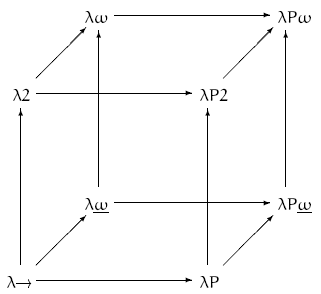
\includegraphics[scale=0.6]{Lambda_cube.png}
\end{frame}

\begin{frame}[fragile]{System $F_c$}
  Currently, Haskell as of GHC 7.10.2 doesnot have true type operators.  Achieves type-level programming through \textit{type families} and equalities on \htycon{Types}.  This axis of extension on $\lambda2$ is termed \text{System} $F_c$.
  \ \\
  \pause
  This, plus a \hkind{Kind} system, a handful of \textit{language extensions}, we are ready fake dependent types in Haskell.
\end{frame}

\begin{frame}[fragile]{Teaser}
  Example please:
  \begin{lstlisting}[style=hask]
    data Vec (n :: @dkNat@) a where
      VNil :: Vec @tc0@ a
      (@vc<:@) :: a -> Vec n a -> Vec (n @tf+@ @tc1@) a

    vs :: Vec @tc6@ Int
    vs = 4 @vc<:@ 8 @vc<:@ 15 @vc<:@ 16 @vc<:@ 23 @vc<:@ 42 @vc<:@ VNil
  \end{lstlisting}

  \pause
  Translation$^*$ please:
  \begin{lstlisting}[style=hask]
    enum Vec<@dkNat@ n, A> {
      Vec<@tc0@, n> VNil,
      Vec<n @tf+@ @tc1@, n> VCons(A a, Vec<n, A> va)
    }

    Vec<@tc6@, Int> vs = VCons(4, VCons(8, VCons(15, VCons(16, VCons(23, VCons(42, VNil))))));
  \end{lstlisting}
  \textit{\tiny{(*) supreme looseness and totally made-up syntax}}
\end{frame}


%%%%%%%%%%%%%%%%%%%%%%%%%%%%%%%%%%%%%%%%%%%%%%%%%%%%%%%%%%%%%%%%%%%%%%%%%%%%%%%%
%%% Dependent type programming in Haskell
%%%%%%%%%%%%%%%%%%%%%%%%%%%%%%%%%%%%%%%%%%%%%%%%%%%%%%%%%%%%%%%%%%%%%%%%%%%%%%%%
\section{Steps toward Dependent Types}

%%%%%%%%%%%%%%%%%%%%%%%%%%%%%%%%%%%%%%%%%%%%%%%%%%%%%%%%%%%%%%%%%%%%%%%%%%%%%%%%
\subsection{Kinds}
\begin{frame}[fragile]{Kinds}
\end{frame}


%%%%%%%%%%%%%%%%%%%%%%%%%%%%%%%%%%%%%%%%%%%%%%%%%%%%%%%%%%%%%%%%%%%%%%%%%%%%%%%%
\subsection{Language Extensions}

\begin{frame}[fragile]{GADTs}
\end{frame}

\begin{frame}[fragile]{KindSignatures}
\end{frame}

\begin{frame}[fragile]{ConstraintKinds}
\end{frame}

\begin{frame}[fragile]{Type Operators}
\end{frame}

\begin{frame}[fragile]{DataKinds}
\end{frame}

\begin{frame}[fragile]{Type Families}
\end{frame}


%%%%%%%%%%%%%%%%%%%%%%%%%%%%%%%%%%%%%%%%%%%%%%%%%%%%%%%%%%%%%%%%%%%%%%%%%%%%%%%%
%%% Q & A
%%%%%%%%%%%%%%%%%%%%%%%%%%%%%%%%%%%%%%%%%%%%%%%%%%%%%%%%%%%%%%%%%%%%%%%%%%%%%%%%
\section{Questions}

% q&a
\begin{frame}
  Questions?
\end{frame}


\end{document}

